\begin{figure*}[t]
\centering
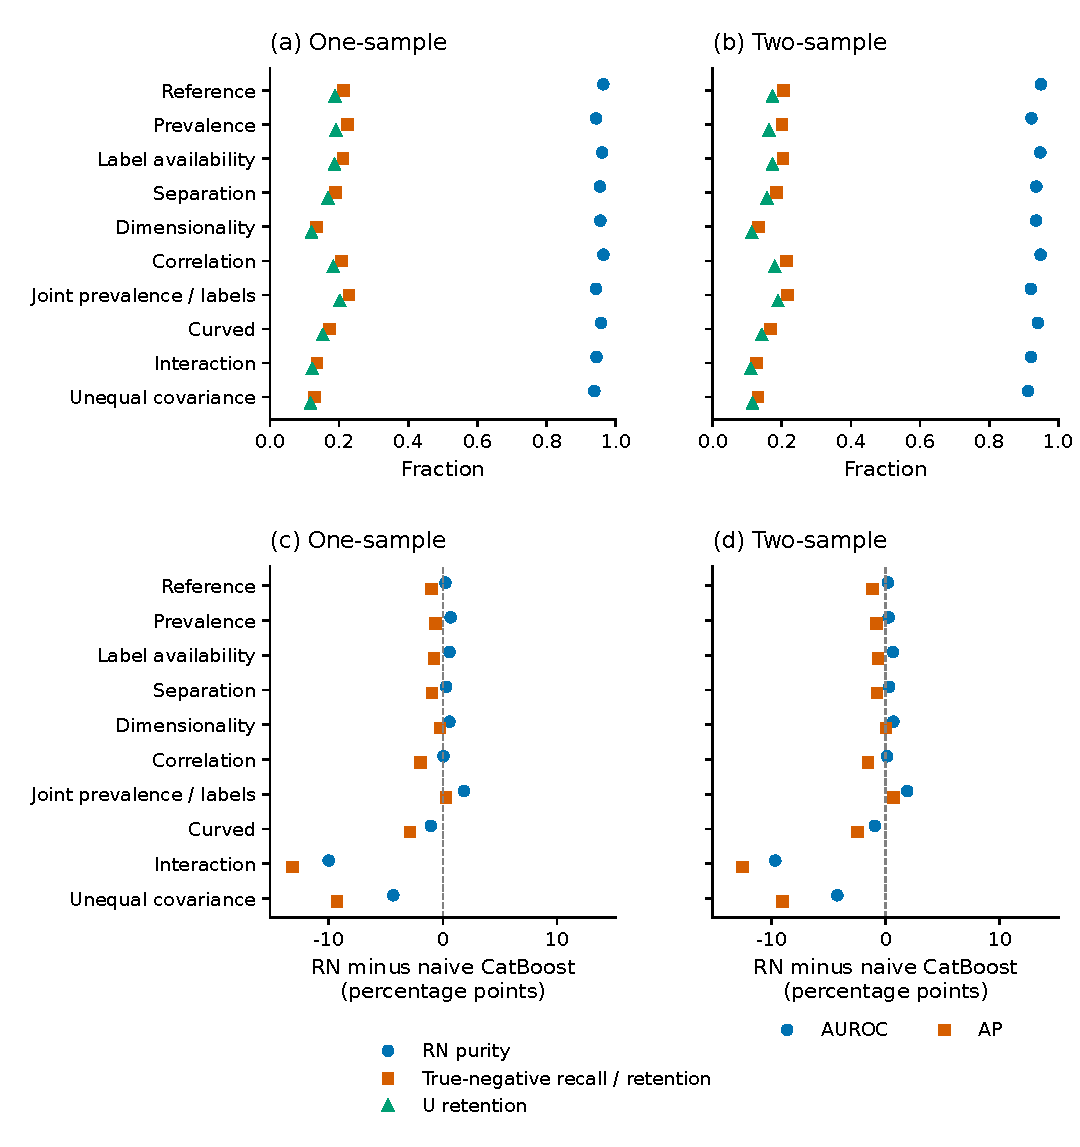
\includegraphics[page=1,width=\textwidth]{mlj_revision/display_package/supplement/figures/fig_s_rn_mechanism.pdf}
\caption{RN masks were reconstructed from exact archived data/code because selected indices were not originally stored. CatBoost results use the final train+validation RN selection stage. RN purity is true negatives / selected U; true-negative recall is selected true negatives / available true negatives (also the fraction of available true negatives retained). U retention is selected U / available U and is shown separately. The figure averages settings within each of ten families; the table retains all 40 settings per design. Interaction is explicitly labelled. AUROC/AP changes are RN CatBoost minus naive CatBoost; no broad BA comparison is made. RN CatBoost: negative-set quality and ranking changes. Ten design-defined families; settings are equally weighted within each family. True-negative recall and the fraction of available true negatives retained are the same quantity.}
\label{fig:fig-s-rn-mechanism-page1}
\end{figure*}
